\documentclass{beamer}
\usepackage{amsmath}
\usepackage{hyperref}
\usepackage{listings}
\usepackage{xcolor}
\hypersetup{colorlinks=true, citecolor=blue, filecolor=blue, linkcolor=blue, urlcolor=blue}
\definecolor{codegreen}{rgb}{0,0.6,0}
\definecolor{codegray}{rgb}{0.5,0.5,0.5}
\definecolor{codepurple}{rgb}{0.58,0,0.82}
\definecolor{backcolour}{rgb}{0.95,0.95,0.92}
 
\lstdefinestyle{mystyle}{
    backgroundcolor=\color{backcolour},   
    commentstyle=\color{codegreen},
    keywordstyle=\color{magenta},
    numberstyle=\tiny\color{codegray},
    stringstyle=\color{codepurple},
    basicstyle=\ttfamily\footnotesize,
    breakatwhitespace=false,         
    breaklines=true,                 
    captionpos=b,                    
    keepspaces=true,                 
    %numbers=left,                    
    numbersep=5pt,                  
    showspaces=false,                
    showstringspaces=false,
    showtabs=false,                  
    tabsize=2
}
 
\lstset{style=mystyle}

\mode<presentation> {

% The Beamer class comes with a number of default slide themes
% which change the colors and layouts of slides. Below this is a list
% of all the themes, uncomment each in turn to see what they look like.

%\usetheme{default}
\usetheme{AnnArbor}
%\usetheme{Antibes}
%\usetheme{Bergen}
%\usetheme{Berkeley}
%\usetheme{Berlin}
%\usetheme{Boadilla}
%\usetheme{CambridgeUS}
%\usetheme{Copenhagen}
%\usetheme{Darmstadt}
%\usetheme{Dresden}
%\usetheme{Frankfurt}
%\usetheme{Goettingen}
%\usetheme{Hannover}
%\usetheme{Ilmenau}
%\usetheme{JuanLesPins}
%\usetheme{Luebeck}
%\usetheme{Madrid}
%\usetheme{Malmoe}
%\usetheme{Marburg}
%\usetheme{Montpellier}
%\usetheme{PaloAlto}
%\usetheme{Pittsburgh}
%\usetheme{Rochester}
%\usetheme{Singapore}
%\usetheme{Szeged}
%\usetheme{Warsaw}

% As well as themes, the Beamer class has a number of color themes
% for any slide theme. Uncomment each of these in turn to see how it
% changes the colors of your current slide theme.

%\usecolortheme{albatross}
%\usecolortheme{beaver}
%\usecolortheme{beetle}
%\usecolortheme{crane}
%\usecolortheme{dolphin}
%\usecolortheme{dove}
%\usecolortheme{fly}
%\usecolortheme{lily}
%\usecolortheme{orchid}
%\usecolortheme{rose}
%\usecolortheme{seagull}
%\usecolortheme{seahorse}
%\usecolortheme{whale}
%\usecolortheme{wolverine}

%\setbeamertemplate{footline} % To remove the footer line in all slides uncomment this line
\setbeamertemplate{footline}[page number] % To replace the footer line in all slides with a simple slide count uncomment this line

\setbeamertemplate{navigation symbols}{} % To remove the navigation symbols from the bottom of all slides uncomment this line
}

\usepackage{graphicx} % Allows including images
\usepackage{booktabs} % Allows the use of \toprule, \midrule and \bottomrule in tables
%\usepackage {tikz}
\usepackage{tkz-graph}
\GraphInit[vstyle = Shade]
\tikzset{
  LabelStyle/.style = { rectangle, rounded corners, draw,
                        minimum width = 2em, fill = yellow!50,
                        text = red, font = \bfseries },
  VertexStyle/.append style = { inner sep=5pt,
                                font = \normalsize\bfseries},
  EdgeStyle/.append style = {->, bend left} }
\usetikzlibrary {positioning}
%\usepackage {xcolor}
\definecolor {processblue}{cmyk}{0.96,0,0,0}
%----------------------------------------------------------------------------------------
%	TITLE PAGE
%----------------------------------------------------------------------------------------

\title[Local Descent]{Numerical Optimization 04: Local Descent} % The short title appears at the bottom of every slide, the full title is only on the title page

\author{Qiang Zhu} % Your name
\institute[University of Nevada Las Vegas] % Your institution as it will appear on the bottom of every slide, may be shorthand to save space
{
University of Nevada Las Vegas\\ % Your institution for the title page
\medskip
}
\date{\today} % Date, can be changed to a custom date

\begin{document}

\begin{frame}
\titlepage % Print the title page as the first slide
\end{frame}

\begin{frame}
\frametitle{Overview} % Table of contents slide, comment this block out to remove it
\tableofcontents % Throughout your presentation, if you choose to use \section{} and \subsection{} commands, these will automatically be printed on this slide as an overview of your presentation
\end{frame}

%----------------------------------------------------------------------------------------
%	PRESENTATION SLIDES
%----------------------------------------------------------------------------------------

%------------------------------------------------

\section{A general model for optimization}
\begin{frame}{Optimization involving multivariate functions}
Similar to the single variable function, a common approach to optimization is to incrementally improve a design point $x$ by taking a step that minimizes the objective value based on a local model. The local model may be obtained, for example, from a first- or second-order Taylor approximation.
\begin{itemize}
    \item Check whether $x_k$ satisfies the termination conditions. If it does, terminate; otherwise proceed to the next step.
    \item Determine the descent direction $d_k$ using local information such as the gradient or Hessian. 
    \item Determine the step size or learning rate $\alpha_k$.
    \item Compute the next design point according to:
    \begin{equation*}
        x_{k+1} = x_k + \alpha_k d_k
    \end{equation*}
\end{itemize}

\end{frame}

\section{Line Search}
\begin{frame}{Line Search}
Assuming that we have chosen a descent direction $d$. We need to choose the step factor $\alpha$ to obtain our next design point. One approach is to use \textcolor{blue}{line search}, which selects the step factor that minimizes the one-dimensional function:
\begin{equation*}
    \underset{\alpha}{\textrm{minimize}}: f(x+\alpha d)
\end{equation*}

Line search is a univariate optimization problem, which was covered in the previous lecture. We can apply the univariate optimization method of our choice. To inform the search, we can use the \textcolor{blue}{derivative} of the line search objective, which is simply the directional derivative along $d$ at $x + \alpha d$.\\

One needs to be cautious in choosing $\alpha$. Large steps will result in faster convergence but risk overshooting the minimum. Smaller steps is more stable but very slow. A fixed step factor $\alpha$ is sometimes referred to as a learning rate.

\end{frame}


\begin{frame}{Approximate line search}
It is often more computationally efficient to perform more iterations of a descent method than to do exact line search at each iteration. In this case, the goal is to \textcolor{blue}{find a suitable step size with a small number of evaluations}.

Ideally, it needs to satisfy the following

\begin{itemize}
    \item Sufficient decrease
    \begin{equation*}
        f(x^{k+1}) \leq f(x^k) + \beta\alpha \nabla _{d^k} f(x^k)
    \end{equation*}
    \item Curvature condition
    \begin{equation*}
        \nabla _{d^k} f(x^{k+1}) \geq \sigma \nabla _{d^k} f(x^k)
    \end{equation*}
\end{itemize}


\end{frame}

\begin{frame}{Sufficient decrease}
    \begin{equation*}
        f(x^{k+1}) \leq f(x^k) + \beta\alpha \nabla _{d^k} f(x^k)
    \end{equation*}
    
where $\beta \in [0, 1]$. A common choice is 1e-4.  
\begin{figure}
\centering
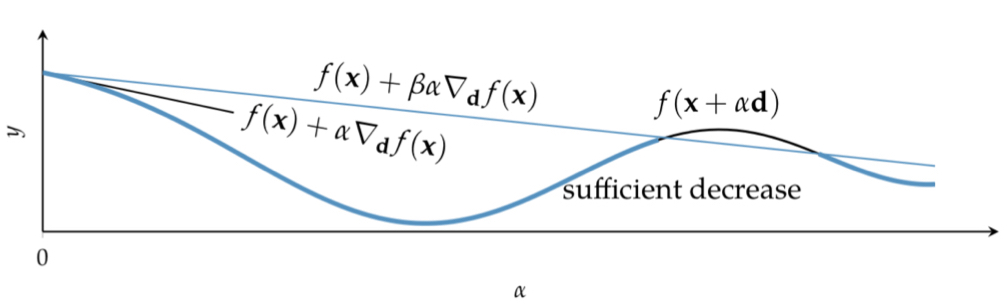
\includegraphics[width=120mm]{Figs/sufficient_decrease.jpeg}
\end{figure}

\textcolor{blue}{Question: what will happen if you adjust $\beta$?}
\end{frame}

\begin{frame}{Curvature condition}
    \begin{equation*}
        \nabla _{d^k} f(x^{k+1}) \geq \sigma \nabla _{d^k} f(x^k)
    \end{equation*}
where $\sigma$ controls how shallow the next directional derivative must be.
It is common to set $\beta < \sigma < 1$ with $\sigma$ = 0.1 in the conjugate gradient method and 0.9 in Newton’s method.
\begin{figure}
\centering
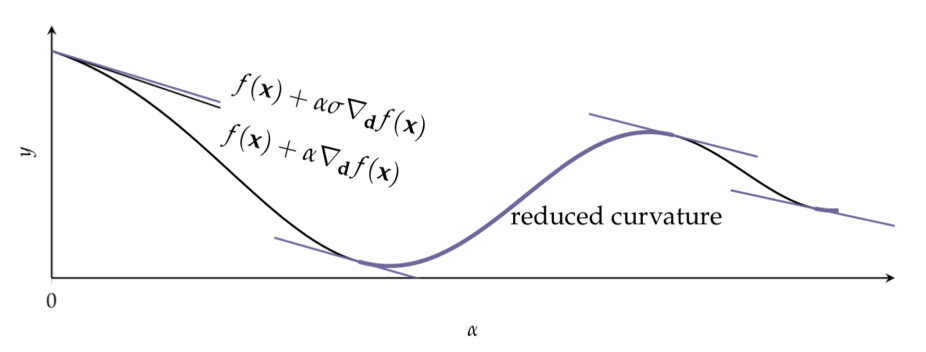
\includegraphics[width=120mm]{Figs/curvature1.jpeg}
\end{figure}
\end{frame}


\begin{frame}{More restrictive curvature condition (strong Wolfe)}
    \begin{equation*}
        |\nabla _{d^k} f(x^{k+1})| \leq -\sigma \nabla _{d^k} f(x^k)
    \end{equation*}
where $\sigma$ controls how shallow the next directional derivative must be.
It is common to set $\beta < \sigma < 1$ with $\sigma$ = 0.1 in the conjugate gradient method and 0.9 in Newton’s method.
\begin{figure}
\centering
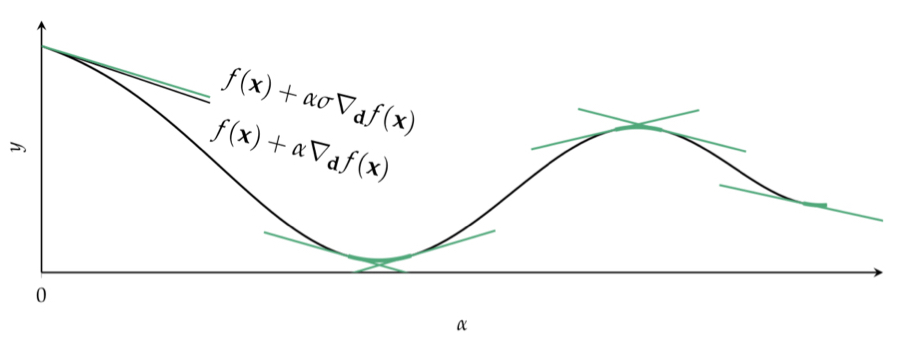
\includegraphics[width=120mm]{Figs/curvature2.jpeg}
\end{figure}
\end{frame}

\begin{frame}{When both conditions are applied}
\begin{figure}
\centering
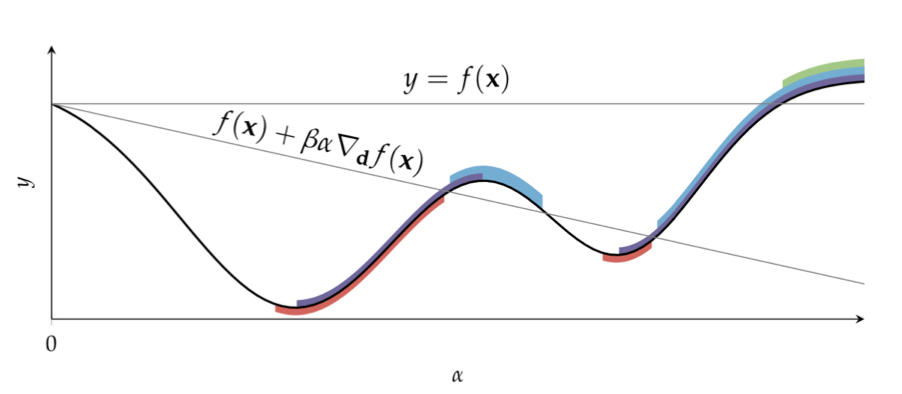
\includegraphics[width=120mm]{Figs/two-conditions.jpeg}
\end{figure}
\end{frame}

\section{A practical line search}
\begin{frame}{Graphical illustration of line search}

\begin{itemize}
    \item Initial Bracket
    \item Fibonacci/0.618/bisection until it satisfies the conditions
\end{itemize}

\begin{figure}
\centering
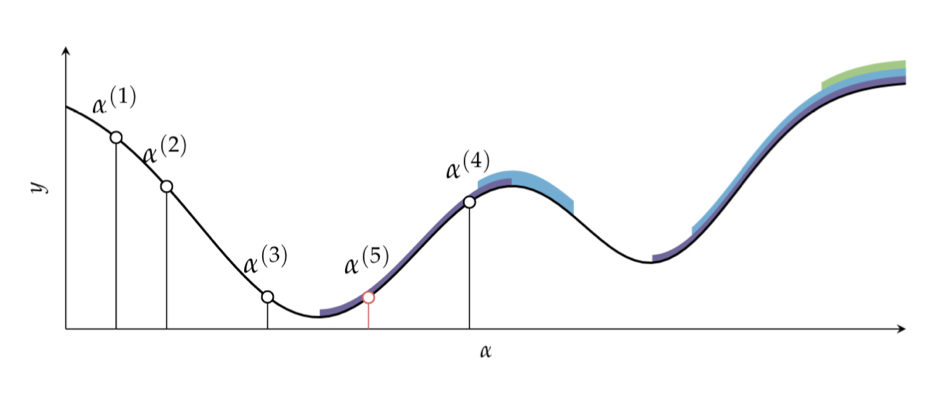
\includegraphics[width=120mm]{Figs/linesearch.jpeg}
\end{figure}

\end{frame}

\begin{frame}{Terminations conditions}
\begin{itemize}
    \item Maximum iterations.
    \item Absolute improvement. If the change is smaller than a given threshold, it will terminate:
    \begin{equation*}
        f(x_k) - f(x_{k+1}) < \epsilon_a
    \end{equation*}
    
    \item Relative improvement. If the change is smaller than a given threshold, it will terminate:
    \begin{equation*}
        f(x_k) - f(x_{k+1}) < \epsilon_r |f(x_k)|
    \end{equation*}
    
    \item Gradient magnitude. We can also terminate based on the magnitude of the gradient:
        \begin{equation*}
            |\nabla f(x_{k+1})| < \epsilon_g 
        \end{equation*}
\end{itemize}

\end{frame}



\section{Summary}
\begin{frame}{Summary}
    \begin{itemize}
        \item Descent direction methods incrementally descend toward a local optimum.
        \item Univariate optimization can be applied during line search.
        \item Approximate line search can be used to identify appropriate descent step sizes.
        \item Termination conditions for descent methods can be based on multiple criteria
    \end{itemize}
\end{frame}
\end{document}

